\section{Kiến thức cơ sở}
\subsection{Mục tiêu chương}
Sau khi hoàn thành chương này, người học có thể:
\begin{itemize}
    \item \textbf{Nắm vững lý thuyết nền tảng:} Cung cấp định nghĩa, cách xác định và phân tích cực trị của hàm trùng phương $y = ax^4 + bx^2 + c$ ($a \neq 0$).
    \item \textbf{Hiểu rõ hình học đồ thị:} Nhận biết các dạng đồ thị tiêu biểu của hàm trùng phương dựa vào dấu của các hệ số $a$ và $b$.
    \item \textbf{Khai thác các tính chất quan trọng:} Hệ thống hóa các tính chất hình học và đại số đặc trưng của hàm trùng phương, làm cơ sở cho việc chứng minh bản chất của các công thức tính nhanh ở các phần tiếp theo.
\end{itemize}
\vspace{0.5cm}
Trong giải tích, nhiều hàm số không chỉ mô tả sự biến thiên của các lượng thực tế mà còn sở hữu những đặc tính đối xứng hình học rất đặc trưng. Dù hệ số của hàm số thay đổi, hình dáng đồ thị của chúng vẫn tuân theo những dạng hình học tiêu chuẩn (dạng chữ U hoặc chữ W/M).

Ví dụ, khi xét hàm số bậc bốn chỉ chứa các số mũ chẵn $y = ax^4 + bx^2 + c$, đồ thị của nó luôn nhận trục tung $Oy$ làm trục đối xứng. Tùy thuộc vào dấu của các hệ số $a$ và $b$, số lượng và vị trí các điểm cực trị sẽ thay đổi nhưng luôn tạo thành những cấu trúc hình học có tính quy luật rõ rệt (như tam giác cân hoặc tam giác vuông).

Trong chương này, ta sẽ hệ thống hóa các kiến thức cơ bản nhất về hàm trùng phương: tập xác định, sự biến thiên, các dạng đồ thị tiêu biểu và các bài toán liên quan đến cực trị của hàm trùng phương.

% ============================================================

\subsection{Hàm trùng phương và cực trị}

\subsubsection{Hàm trùng phương}

\textbf{Định nghĩa:} 
Hàm trùng phương là một trường hợp đặc biệt của hàm số bậc bốn tổng quát $y = ax^4 + bx^3 + cx^2 + dx + e$ ($a \neq 0$) khi các hệ số của bậc lẻ đều bằng $0$ ($b = 0, d = 0$). 

Dạng tổng quát của hàm trùng phương là:
\[ y = ax^4 + bx^2 + c \quad (a \neq 0) \]

\textbf{Ví dụ 1 (Ví dụ về hàm trùng phương):}
Các hàm số sau đây là hàm trùng phương:
\begin{itemize}
    \item $y = x^4 - 2x^2 + 3$ (với $a = 1, b = -2, c = 3$)
    \item $y = -2x^4 + 5x^2$ (với $a = -2, b = 5, c = 0$)
    \item $y = 3x^4 - 1$ (với $a = 3, b = 0, c = -1$)
    \item $y = -x^4$ (với $a = -1, b = 0, c = 0$)
\end{itemize}

\textbf{Ví dụ 2 (Ví dụ không phải hàm trùng phương):}
Các hàm số sau đây \textbf{không phải} là hàm trùng phương:
\begin{itemize}
    \item $y = x^4 - 3x^3 + 2x^2 - 1$ (vì chứa số mũ lẻ $x^3$, đây là hàm bậc bốn tổng quát).
    \item $y = 0x^4 + 2x^2 + 1 \iff y = 2x^2 + 1$ (vì hệ số $a = 0$, đây là hàm bậc hai).
    \item $y = x^4 + \dfrac{1}{x^2}$ (vì chứa biến $x$ ở mẫu thức, không phải hàm đa thức).
\end{itemize}

\textbf{Nhận xét:}
\begin{itemize}
    \item Vì chỉ chứa các số mũ chẵn của biến $x$, hàm trùng phương là một \textbf{hàm số chẵn}.
   
\end{itemize}

\subsubsection{Cực trị của hàm trùng phương}


Cho hàm trùng phương $y = ax^4 + bx^2 + c \quad (a \neq 0)$.

\textbf{1. Định nghĩa và Tập xác định:}
\begin{itemize}
    \item Tập xác định: $D = \mathbb{R}$.
    \item Đạo hàm: $y' = 4ax^3 + 2bx = 2x(2ax^2 + b)$.
\end{itemize}

\textbf{2. Điều kiện tồn tại và số lượng điểm cực trị:}

Xét phương trình:
\[ y' = 0 \iff 2x(2ax^2 + b) = 0 \iff \left[\begin{array}{l} x = 0 \\ 2ax^2 + b = 0 \quad (1) \end{array}\right. \]

\begin{itemize}
    \item \textbf{Trường hợp 1 (Hàm số có 3 điểm cực trị):} \\
    Phương trình (1) có hai nghiệm phân biệt khác $0$, điều này xảy ra khi và chỉ khi:
    \[ a \cdot b < 0 \]
    Khi đó, đồ thị hàm số có 3 điểm cực trị là:
    \[ A(0; c), \quad B\left(-\sqrt{-\frac{b}{2a}}; c - \frac{b^2}{4a}\right), \quad C\left(\sqrt{-\frac{b}{2a}}; c - \frac{b^2}{4a}\right) \]
    \textit{Nhận xét:} Ba điểm cực trị $A, B, C$ luôn tạo thành một tam giác cân tại đỉnh $A$ (nằm trên trục $Oy$).
    
\end{itemize}
\begin{itemize}
    \item \textbf{Trường hợp 2 (Hàm số có 1 điểm cực trị):} \\
    Phương trình (1) vô nghiệm hoặc có nghiệm kép $x = 0$, điều này xảy ra khi và chỉ khi:
    \[ a \cdot b \geq 0 \]
    Khi đó, hàm số chỉ có duy nhất $1$ điểm cực trị tại $x = 0$ (tọa độ điểm cực trị là $A(0; c)$).
\begin{figure}[htbp]
    \centering
    \begin{tikzpicture}
        \begin{axis}[
            title = {\textbf{Ví dụ 1: Đồ thị hàm số $y = x^4 - 2x^2 + 1$ ($a\cdot b < 0$)}},
            axis lines = middle,
            xlabel = {$x$},
            ylabel = {$y$},
            xmin = -1.8, xmax = 1.8,
            ymin = -0.5, ymax = 2.5,
            ticks = none,
            enlargelimits = false
        ]
            % Vẽ đồ thị
            \addplot [domain=-1.6:1.6, samples=100, smooth, thick, blue] {x^4 - 2*x^2 + 1};
            
            % Đánh dấu các điểm cực trị
            \node[above right] at (axis cs:0,1) {$A(0;1)$};
            \node[below left] at (axis cs:-1,0) {$B(-1;0)$};
            \node[below right] at (axis cs:1,0) {$C(1;0)$};
            \filldraw[red] (axis cs:0,1) circle (1.5pt);
            \filldraw[red] (axis cs:-1,0) circle (1.5pt);
            \filldraw[red] (axis cs:1,0) circle (1.5pt);
        \end{axis}
    \end{tikzpicture}
    \caption{Đồ thị hàm trùng phương có 3 điểm cực trị}
\end{figure}


  
\end{itemize}
\begin{figure}[htbp]
    \centering
    \begin{tikzpicture}
        \begin{axis}[
            title = {\textbf{Ví dụ 2: Đồ thị hàm số $y = x^4 + 2x^2 + 1$ ($a\cdot b \ge 0$)}},
            axis lines = middle,
            xlabel = {$x$},
            ylabel = {$y$},
            xmin = -1.8, xmax = 1.8,
            ymin = -0.5, ymax = 3.5,
            ticks = none,
            enlargelimits = false
        ]
            % Vẽ đồ thị
            \addplot [domain=-1.3:1.3, samples=100, smooth, thick, red] {x^4 + 2*x^2 + 1};
            
            % Đánh dấu điểm cực trị duy nhất
            \node[above right] at (axis cs:0,1) {$A(0;1)$};
            \filldraw[blue] (axis cs:0,1) circle (1.5pt);
        \end{axis}
    \end{tikzpicture}
    \caption{Đồ thị hàm trùng phương có 1 điểm cực trị}
\end{figure}
      
   

% ============================================================
% 1.2.3. ĐỒ THỊ HÀM TRÙNG PHƯƠNG
% ============================================================

\subsection{Đồ thị hàm trùng phương}

Hàm trùng phương có dạng
\[
y=ax^4+bx^2+c,\qquad a\neq 0.
\]

\subsubsection{Đặc điểm của đồ thị hàm trùng phương}

\begin{itemize}
    \item Đồ thị hàm trùng phương đối xứng qua trục tung. Thật vậy,
    \[
    f(-x)
    =a(-x)^4+b(-x)^2+c
    =ax^4+bx^2+c
    =f(x).
    \]
    Do đó, hàm số là hàm chẵn và đồ thị nhận trục $Oy$ làm trục đối xứng.

    \item Tập xác định của hàm số là
    \[
    D=\mathbb{R}.
    \]

    \item Đồ thị hàm trùng phương có thể có tối đa ba điểm cực trị, gồm:
    \begin{itemize}
        \item hai điểm cực tiểu và một điểm cực đại;
        \item hoặc hai điểm cực đại và một điểm cực tiểu.
    \end{itemize}

    \item Khi có ba điểm cực trị, hai điểm cực trị khác $x=0$ có hoành độ đối nhau:
    \[
    x_1=-\sqrt{-\frac{b}{2a}},
    \qquad
    x_2=\sqrt{-\frac{b}{2a}}.
    \]
\end{itemize}


\subsubsection{Các bước khảo sát và vẽ đồ thị hàm trùng phương}

\paragraph{Bước 1. Tìm tập xác định}

Vì hàm trùng phương là một đa thức nên hàm số xác định với mọi
$x\in\mathbb{R}$. Do đó,
\[
D=\mathbb{R}.
\]

\paragraph{Bước 2. Tính đạo hàm và tìm các điểm cực trị}

Ta có
\[
y'=4ax^3+2bx
=2x(2ax^2+b).
\]

Giải phương trình $y'=0$:
\[
2x(2ax^2+b)=0
\]
\[
\Leftrightarrow
x=0
\quad\text{hoặc}\quad
x^2=-\frac{b}{2a}.
\]

Nếu $ab<0$, phương trình có hai nghiệm
\[
x_1=-\sqrt{-\frac{b}{2a}},
\qquad
x_2=\sqrt{-\frac{b}{2a}},
\]
kết hợp với $x=0$, hàm số có ba điểm tới hạn.

Nếu $ab\geq 0$, phương trình
\[
x^2=-\frac{b}{2a}
\]
không có nghiệm thực khi $ab>0$, còn khi $b=0$ thì nghiệm $x=0$
trùng với nghiệm đã có. Vì vậy, hàm số chỉ có một điểm cực trị tại
$x=0$.


\paragraph{Bước 3. Tính đạo hàm cấp hai}

Ta có
\[
y''=12ax^2+2b.
\]

Giải phương trình $y''=0$:
\[
12ax^2+2b=0
\]
\[
\Leftrightarrow
x^2=-\frac{b}{6a}.
\]

Nếu $ab<0$, phương trình có hai nghiệm
\[
x=\pm\sqrt{-\frac{b}{6a}}.
\]

Nếu $ab>0$, phương trình $y''=0$ vô nghiệm.


\paragraph{Bước 4. Lập bảng biến thiên và vẽ đồ thị}

Dựa vào dấu của $y'$ để xác định các khoảng đồng biến,
nghịch biến và các điểm cực trị. Kết hợp với tính đối xứng qua
trục $Oy$, các điểm cực trị, điểm uốn và giao điểm với các trục
tọa độ để phác họa đồ thị.


% ============================================================
% TRƯỜNG HỢP 1
% ============================================================

\subsubsection*{Trường hợp 1: $a > 0, b < 0$ (Hàm số có 3 điểm cực trị)}

% 1. Bảng biến thiên
\begin{center}
\begin{tikzpicture}
   \tkzTabInit[lgt=1.5,espcl=2]{$x$ /1, $y'$ /1, $y$ /2}{$-\infty$, $-\sqrt{-\frac{b}{2a}}$, $0$, $\sqrt{-\frac{b}{2a}}$, $+\infty$}
   \tkzTabLine{, -, 0, +, 0, -, 0, +, }
   \tkzTabVar{+/ $+\infty$, -/ $y_{CT}$, +/ $y_{C Đ}$, -/ $y_{CT}$, +/ $+\infty$}
\end{tikzpicture}
\captionof{figure}{Bảng biến thiên trường hợp $a > 0, b < 0$}
\end{center}

% 2. Đồ thị
\begin{center}
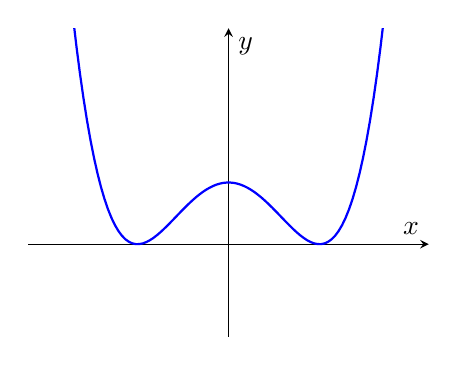
\begin{tikzpicture}
    \begin{axis}[
        width=0.55\textwidth, height=5.5cm,
        axis lines = middle,
        xlabel = {$x$}, ylabel = {$y$},
        xmin = -2.2, xmax = 2.2,
        ymin = -1.5, ymax = 3.5,
        ticks = none,
        enlargelimits = false
    ]
        \addplot[thick, blue, domain=-1.9:1.9, samples=100] {x^4 - 2*x^2 + 1};
    \end{axis}
\end{tikzpicture}
\captionof{figure}{Đồ thị hàm số $y = x^4 - 2x^2 + 1$}
\end{center}

% ============================================================
% TRƯỜNG HỢP 2
% ============================================================

\subsubsection*{Trường hợp 2: $a < 0, b > 0$ (Hàm số có 3 điểm cực trị)}

% 1. Bảng biến thiên
\begin{center}
\begin{tikzpicture}
   \tkzTabInit[lgt=1.5,espcl=2]{$x$ /1, $y'$ /1, $y$ /2}{$-\infty$, $-\sqrt{-\frac{b}{2a}}$, $0$, $\sqrt{-\frac{b}{2a}}$, $+\infty$}
   \tkzTabLine{, +, 0, -, 0, +, 0, -, }
   \tkzTabVar{-/ $-\infty$, +/ $y_{CĐ}$, -/ $y_{CT}$, +/ $y_{CĐ}$, -/ $-\infty$}
\end{tikzpicture}
\captionof{figure}{Bảng biến thiên trường hợp $a < 0, b > 0$}
\end{center}

% 2. Đồ thị
\begin{center}
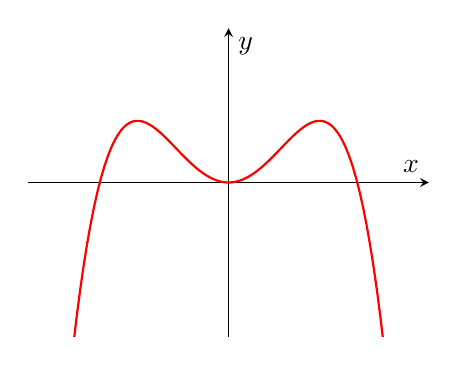
\begin{tikzpicture}
    \begin{axis}[
        width=0.55\textwidth, height=5.5cm,
        axis lines = middle,
        xlabel = {$x$}, ylabel = {$y$},
        xmin = -2.2, xmax = 2.2,
        ymin = -2.5, ymax = 2.5,
        ticks = none,
        enlargelimits = false
    ]
        \addplot[thick, red, domain=-1.9:1.9, samples=100] {-x^4 + 2*x^2};
    \end{axis}
\end{tikzpicture}
\captionof{figure}{Đồ thị hàm số $y = -x^4 + 2x^2$}
\end{center}

% ============================================================
% TRƯỜNG HỢP 3
% ============================================================

\subsubsection*{Trường hợp 3: $a > 0, b \ge 0$ (Hàm số có 1 điểm cực trị)}

% 1. Bảng biến thiên
\begin{center}

\begin{tikzpicture}
   \tkzTabInit[lgt=1.5,espcl=2.5]{$x$ /1, $y'$ /1, $y$ /2}{$-\infty$, $0$, $+\infty$}
   \tkzTabLine{, -, 0, +, }
   \tkzTabVar{+/ $+\infty$, -/ $y_{CT}$, +/ $+\infty$}
\end{tikzpicture}
\captionof{figure}{Bảng biến thiên trường hợp $a > 0, b \ge 0$}
\end{center}

% 2. Đồ thị
\begin{center}
\begin{tikzpicture}
    \begin{axis}[
        width=0.55\textwidth, height=5.5cm,
        axis lines = middle,
        xlabel = {$x$}, ylabel = {$y$},
        xmin = -2, xmax = 2,
        ymin = -0.5, ymax = 3.5,
        ticks = none,
        enlargelimits = false
    ]
        \addplot[thick, blue, domain=-1.7:1.7, samples=100] {x^4 + 0.5*x^2 + 0.5};
    \end{axis}
\end{tikzpicture}
\captionof{figure}{Đồ thị hàm số $y = x^4 + 2x^2 + 1$}
\end{center}
% ============================================================
% TRƯỜNG HỢP 4
% ============================================================

\subsubsection*{Trường hợp 4: $a < 0, b \le 0$ (Hàm số có 1 điểm cực trị)}

% 1. Bảng biến thiên
\begin{center}
\begin{tikzpicture}
   \tkzTabInit[lgt=1.5,espcl=2.5]{$x$ /1, $y'$ /1, $y$ /2}{$-\infty$, $0$, $+\infty$}
   \tkzTabLine{, +, 0, -, }
   \tkzTabVar{-/ $-\infty$, +/ $y_{CĐ}$, -/ $-\infty$}
\end{tikzpicture}
\captionof{figure}{Bảng biến thiên trường hợp $a < 0, b \le 0$}
\end{center}

% 2. Đồ thị
\begin{center}
\begin{tikzpicture}
    \begin{axis}[
        width=0.55\textwidth, height=5.5cm,
        axis lines = middle,
        xlabel = {$x$}, ylabel = {$y$},
        xmin = -2, xmax = 2,
        ymin = -3.5, ymax = 1.5,
        ticks = none,
        enlargelimits = false
    ]
        \addplot[thick, red, domain=-1.7:1.7, samples=100] {-x^4 - 0.5*x^2};
    \end{axis}
\end{tikzpicture}
\captionof{figure}{Đồ thị hàm số $y = -x^4 - 2x^2$}
\end{center}
% ============================================================
% TỔNG KẾT
% ============================================================

\subsubsection{Tóm tắt các trường hợp}

Có thể tổng hợp các trường hợp của hàm trùng phương như sau:

\[
\begin{array}{c|c|c}
\text{Điều kiện} & \text{Số điểm cực trị}
& \text{Dạng cực trị}\\
\hline
a>0,\ b<0 & 3 & 2\text{ cực tiểu, }1\text{ cực đại}\\
a<0,\ b>0 & 3 & 2\text{ cực đại, }1\text{ cực tiểu}\\
a>0,\ b\geq0 & 1 & 1\text{ cực tiểu}\\
a<0,\ b\leq0 & 1 & 1\text{ cực đại}
\end{array}
\]
\vspace{0.5cm}
\begin{center}
\begin{tcolorbox}[colback=blue!5!white,colframe=blue!75!black,title=\textbf{Mẹo nhớ nhanh}]
\begin{itemize}
    \item \textbf{Số lượng cực trị:}
    \begin{itemize}
        \item $a \cdot b < 0 \Rightarrow$ Hàm số có \textbf{3 điểm cực trị}.
        \item $a \cdot b \ge 0 \Rightarrow$ Hàm số có \textbf{1 điểm cực trị}.
    \end{itemize}
    \item \textbf{Dạng đồ thị (Dấu của $a$):}
    \begin{itemize}
        \item $a > 0 \Rightarrow$ Nhánh bên phải cùng luôn \textbf{đi lên} ($+\infty$).
        \item $a < 0 \Rightarrow$ Nhánh bên phải cùng luôn \textbf{đi xuống} ($-\infty$).
    \end{itemize}
\end{itemize}
\end{tcolorbox}
\end{center}
\subsection{1.4. Một số tính chất của hàm số trùng phương}

\begin{itemize}
    \item Đồ thị của hàm số $y = ax^4 + bx^2 + c$ ($a \neq 0$) cắt trục hoành tại $4$ điểm phân biệt có hoành độ lập thành cấp số cộng khi phương trình: $aX^2 + bX + c = 0$ có $2$ nghiệm dương phân biệt thỏa $X_1 = 9X_2$.
    
    \item Nếu đồ thị hàm số có ba điểm cực trị thì ba điểm cực trị tạo thành một tam giác cân có đỉnh nằm trên $Oy$.
    
    \item Nếu đường thẳng $d$ là tiếp tuyến của đồ thị thì đường thẳng $d'$ đối xứng với $d$ qua $Oy$ cũng là tiếp tuyến của đồ thị.
\end{itemize}
\vfill


